\chapter{METODOLOGI}
\label{chap:metodologi}

% Ubah bagian-bagian berikut dengan isi dari desain dan implementasi
% Ubah konten-konten berikut sesuai dengan isi dari metodologi

\section{Data dan Peralatan/ Data dan Alat Bantu/ Material }

% Berikut merupakan data dan perlatan yang mendukung pengerjaan Tugas Akhir ini.
\begin{itemize}
	\item [$\bullet$]Dataset berupa gambar bangun datar segitiga, persegi, persegi panjang, lingkaran, dan trapesium berjumlah 50 gambar untuk tiap bangun datar
	
	% \begin{figure} [H] \centering
		%   % Nama dari file gambar yang diinputkan
		%   \includegraphics[scale=0.2]{gambar/UTKFace.png}
		%   % Keterangan gambar yang diinputkan
		%   \caption{Dataset UTKFace}
		%   % Label referensi dari gambar yang diinputkan
		%   \label{fig:UTKFace}
		% \end{figure}
	
	\item [$\bullet$]Dataset berupa gambar tulisan parameter bangun datar 
	\begin{itemize}
		\item [$\bullet$]Untuk bangun datar segitiga parameternya adalah huruf a(alas) dan t(tinggi) berjumlah 50 gambar untuk tiap huruf
		\item [$\bullet$]Untuk bangun datar persegi parameternya adalah huruf s(sisi) berjumlah 50 gambar untuk tiap huruf
		\item [$\bullet$]Untuk bangun datar persegi panjang parameternya adalah huruf P(panjang) dan L(lebar) berjumlah 50 gambar untuk tiap huruf
		\item [$\bullet$]Untuk bangun datar lingkaran parameternya adalah huruf R(jari-jari) berjumlah 50 gambar untuk tiap huruf
		\item [$\bullet$]Untuk bangun datar trapesium parameternya adalah huruf a(sisi atas), b(sisi bawah), dan T(tinggi) berjumlah 50 gambar untuk tiap huruf
		\item [$\bullet$]Angka untuk parameter (1,2,3,4,5,6,7,8,9,0) berjumlah 50 gambar untuk tiap angka
	\end{itemize}
	
	\item [$\bullet$]Roboflow sebagai alat untuk melabeli atau memberikan anotasi pada gambar yang akan digunakan untuk melatih model YOLO.
	\item [$\bullet$]Kamera \\
	
\end{itemize}


\section{Metodologi Penelitian}
% Metodologi yang digunakan dalam pengerjaan Tugas Akhir ini adalah sebagai berikut.
% Contoh input gambar dengan format *.jpg
\begin{figure}[ht]
	% Nama dari file gambar yang diinputkan
	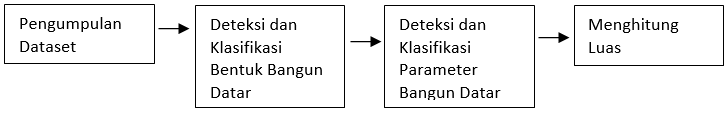
\includegraphics[scale=0.7]{gambar/Metodologi.png}
	% Keterangan gambar yang diinputkan
	\caption{Diagram blok metodologi}
	% Label referensi dari gambar yang diinputkan
	\label{fig:Metodologi}
\end{figure}

\begin{enumerate}
	\item \textbf{Pengumpulan Data} \\
	Pengumpulan dataset dilakukan dengan menggambar bangun datar dan parameter bangun datar pada papan tulis lalu disimpan dalam bentuk foto. lalu melakukan pelabelan pada objek yang ingin dideteksi
	\item \textbf{Deteksi dan Klasifikasi Bentuk Bangun Datar} \\
	Citra diproses dari kamera lalu program akan mendeteksi dan mengklasifikasi bentuk bangun datar.
	\item \textbf{Deteksi dan Klasifikasi Parameter Bangun Datar} \\
	Citra diproses dari kamera lalu program akan mendeteksi dan mengklasifikasi parameter bangun datar..
	\item \textbf{Menghitung Luas} \\
	Dari hasil deteksi dan klasifikasi, program akan melakukan perhitungan luas sebuah bangun datar.
\end{enumerate}





%Penelitian ini dilaksanakan sesuai \lipsum[1][1-5]


%\section{Peralatan}
%\label{sec:peralatan}

%Alat yang digunakan yaitu: \lipsum[1]

%\subsection{Perangkat}
%\label{subsec:perangkat}

%Perangkat yang digunakan menggunakan spesifikasi \lipsum[1]

%\section{Desain Sistem}
%\label{sec:desainsistem}

%Sistem akan dibuat dengan \lipsum[1-2]

% Per blok diagram dijelaskan dan dibuatkan section masing-masing

% \section{Blok Diagram}
% \label{sec:blokdiagram}

% Contoh pembuatan potongan kode
%\begin{lstlisting}[
%  language=C++,
%  caption={Program halo dunia.},
%  label={lst:halodunia}
%]
%#include <iostream>
%
%int main() {
%    std::cout << "Halo Dunia!";
%    return 0;
%}
%\end{lstlisting}

%\lipsum[2-3]

% Contoh input potongan kode dari file
%\lstinputlisting[
%  language=Python,
%  caption={Program perhitungan bilangan prima.},
%  label={lst:bilanganprima}
%]{program/bilangan-prima.py}

%\lipsum[4]
